\documentclass[tikz,border=3mm]{standalone}
\usepackage{amsmath}
\begin{document}

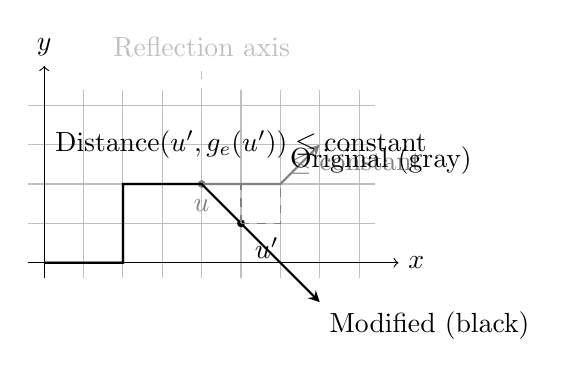
\begin{tikzpicture}[
    pathStyle/.style={thick, -stealth},
    original/.style={pathStyle, gray},
    modified/.style={pathStyle, black},
    reflectionAxis/.style={dashed, gray!50},
    point/.style={circle, fill, inner sep=1pt}
]
    % Coordinate system
    \draw[gray!50, thin, step=0.5] (-0.2, -0.2) grid (4.2, 2.2);
    \draw[->] (-0.2,0) -- (4.5,0) node[right] {$x$};
    \draw[->] (0,-0.2) -- (0,2.5) node[above] {$y$};

    % Original path (gray)
    \draw[original] (0,0) -- (1,0) -- (1,1) -- (2,1) 
        node[point, label=below:$u$] (u) {} -- (3,1) -- (3.5,1.5);
    
    % Reflection axis (vertical line at u.x)
    \draw[reflectionAxis] (u) -- (u |- 0,2.5) node[above] {Reflection axis};
    
    % Modified path (black)
    \draw[modified] (0,0) -- (1,0) -- (1,1) -- (2,1) 
        -- (2.5,0.5) node[point, label=below right:$u'$] (u') {}
        -- (3,0) -- (3.5,-0.5);
    
    % Bounding box for reflection distance
    \draw[dashed, gray] (u') rectangle ++(0.5,0.5) node[above right] {$\leq \text{constant}$};
    
    % Annotations
    \node[above right] at (3,1) {Original (gray)};
    \node[below right] at (3.5,-0.5) {Modified (black)};
    \node at (2.5,1.5) {$\text{Distance}(u', g_e(u')) \leq \text{constant}$};
\end{tikzpicture}

\end{document}